\FloatBarrier
\subsection{Technologies to be developed / R\&D} \label{sec:RD}
%\emph{Author(s): \textbf{K.\ Kokeyama}, S.\ Hild, A.\ Thuering, J.\ Franc, R.\ Nawrodt \\}
\FloatBarrier
\subsubsection{Thermal noise reduction due to LG modes}
\label{sec:thermalnoiseLG}

%\emph{Author(s): K.\ Kokeyama}
Thermal noise will be limiting future generations of interferometric gravitational wave
detectors in the central frequency band (where the detectors are most sensitive). In the case of the xylophone design, the cryogenic LF interferometer benefits from the 
low temperature so that the mirror thermal noise sits well below the quantum noise.
However, in the case of the HF detector, we need to employ additional techniques
to reduce the thermal noise below the ET requirement.
Higher-order Laguerre-Gauss (LG) mode beams
have been proposed and investigated for the reduction of mirror the thermal noise
for the ET-HF interferometer~\cite{Mours06, Vinet2007}.
LG modes are solutions of the paraxial wave equation in cylindrical coordinates,
in a similar way to the Hermite Gaussian modes which are the solutions in Cartesian coordinates.
They have radial power distributions as shown in Fig.~\ref{fig:tech-LG}
which spreads the light power more evenly over the mirror surface (for a given
amount of light lost over the mirror edge) than those of the conventional fundamental mode,
therefore higher-order LG mode beams can be used to reduce the thermal noise
without introducing higher clipping-losses.
%
Also flat-top and conical beams have been proposed
for future gravitational-wave detectors. However
higher-order LG mode beams have the advantage
that they have the spherical wave fronts
and thus are compatible with conventional optics
such as spherical mirrors and lenses.
On the other hand, flat-top and conical beams require non-spherical complex mirrors.
Non-spherical mirrors have been tested so far do not satisfy.
angular alignment requirements~\cite{savov06}.
Also, with current technology it is unclear if these mirrors can be manufactured with
the same surface quality as spherical mirrors for which we have decades of experience.
%Theoretical advantageous number
Previous investigations have shown that implementing LG$_{33}$ modes
in Advanced detectors could increase the inspiral range for NS binaries 
by a factor of two through the reduction of Brownian thermal noise
in comparison to the fundamental LG$_{00}$ mode~\cite{Chelkowski2009}.
%One must be careful of the clipping loss,
%since the power distribution of the LG$_{33}$ mode is larger
%than the LG$_{00}$ for a given beam size parameter.
%
%Note that the thermo-elastic noise may be increased
%because of the periodic intensity patterns of strong and weak,
%however, this does not count as a problem
%because the currently most limiting thermal noise in gravitational-wave detectors
%is the coating Brownian thermal noise.
%
%Simulation results (PD signal/alignment signal)
In addition, higher-order LG beams are fully compatible with the conventional
length and angular sensing signals.
This fact indicates that changing over from the fundamental mode to
the higher-order LG mode should not require any new control strategy.
Ref. \cite{Chelkowski2009} analyzed the control signals using numerical simulation tools
and found that the performance of the LG$_{33}$ beam
in tilt-to-longitudinal phase coupling,
generation of angular control signals, and the corresponding control matrices,
was equivalent to or better than that of the LG$_{00}$ beam.
\begin{figure}
\centering
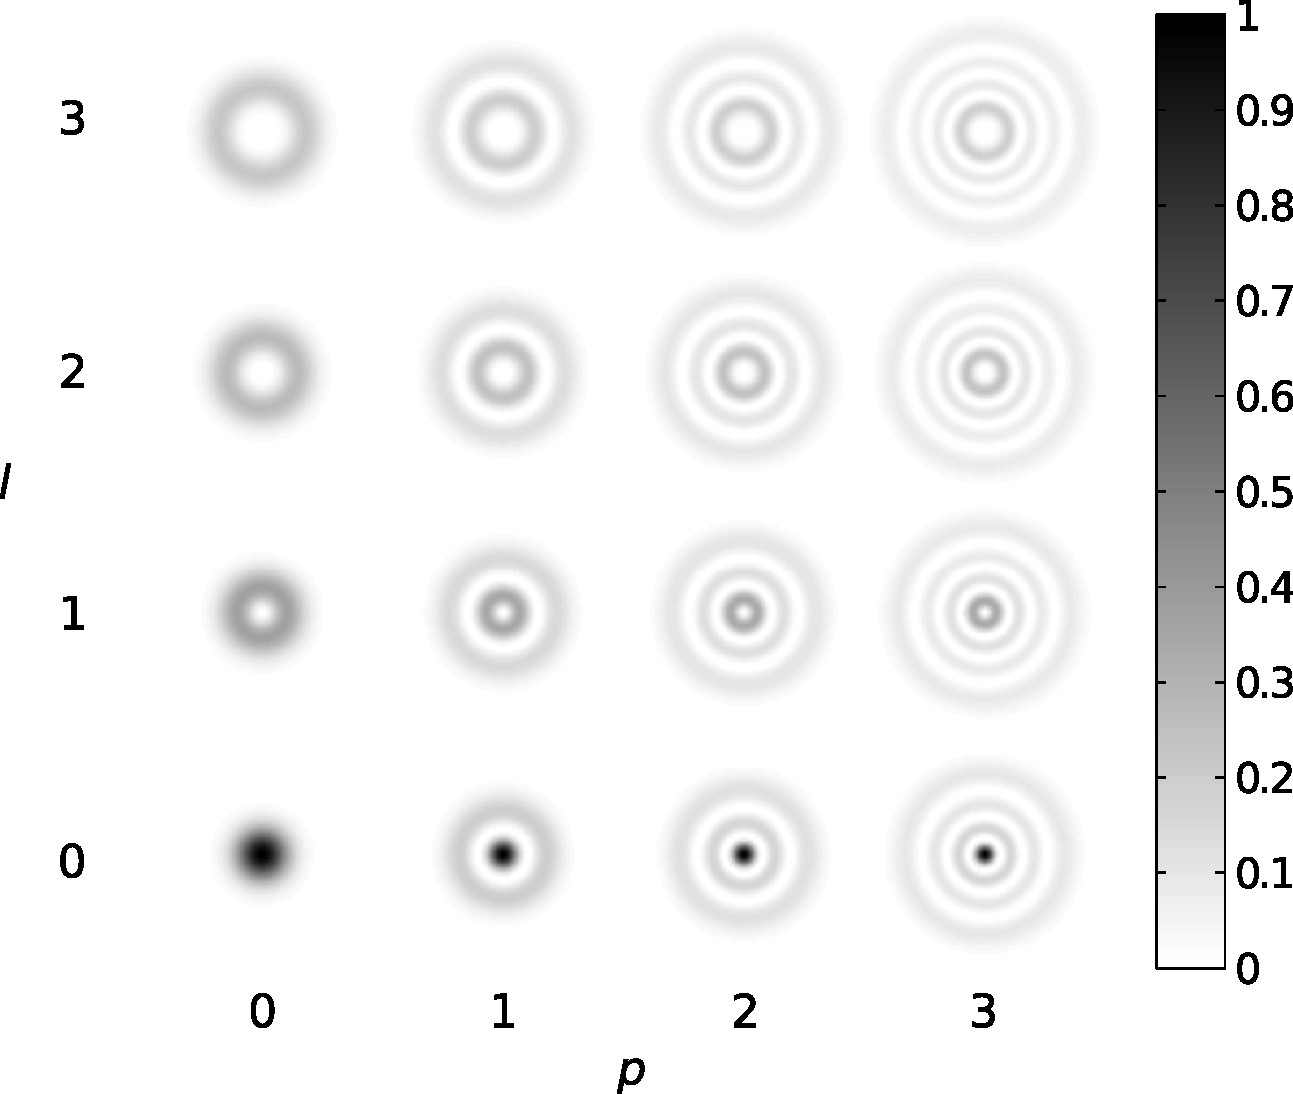
\includegraphics[scale =0.4]{./Sec_Optics/LGintensities33.pdf}
\caption{Power distributions of LG$_{pl}$ mode.
$p$ is the radial mode index ($p\geq0$),
and $l$ is the azimuthal mode index.
The power distribution of LG$_{00}$ mode is equivalent
to that of the conventional TEM$_{00}$ mode.%
} \label{fig:tech-LG}
\end{figure}


%Experimental
LG mode technology for gravitational wave detectors
is currently in a transition phase from the theoretical
and simulation investigation to the experimental investigation phase.
The first table-top experiment has demonstrated the generation of a LG$_{33}$ beam
and the mode cleaner cavity performance with the generated LG$_{33}$ beam \cite{Fulda10}.
The LG$_{33}$ beam was generated by converting the LG$_{00}$ beam to LG$_{33}$ beam
using a computer-controlled liquid-crystal-on-silicon spatial-light modulator (SLM).
The PDH error signal was properly obtained with a LG$_{33}$ beam,
and successfully used to control the longitudinal
degree of freedom of the mode-cleaner cavity.
The mode purity of the generated LG$_{33}$ beam
was increased from 66\% to 99\% upon transmission through the linear mode
cleaner, demonstrating that very high-purity LG$_{33}$ mode
light sources can be produced in this way.
Further experimental investigations, using diffractive optical elements instead of SLM, are underway. A LG33 high-purity beam has been generated with a fused silica diffractive element and a linear mode-cleaner~\cite{Granata10}. The ratio between the powers of the LG00 injected and the high-purity LG33 generated was 36\%. By measuring the transmission of the setup for the LG00, it was possible to infer that the conversion efficiency specific to the LG33 was 49\%. The generated LG33 mode was sent to a table-top Michelson interferometer, locked on the dark fringe. 

However, LG modes pose one new challenge, namely mode degeneracy in 
optical cavities:
Several modes of $(l,p)$ exist with the same order, $2|l|+p$,
and they have identical Gaussian beam parameters, such as radius of curvature and Gouy phase.
Therefore these modes can all resonate in the same cavity,
and can not rejected or cleaned away without adding unwanted complexity to the system, 
such as masks. These modes may contaminate the purity of the desired mode
and may require a higher quality for the mirror surfaces.
This effect does not occur for the fundamental mode, since there is only one mode the in zeroth order. Several research programs are currently underway to investigate 
mode degeneracy with numerical simulations and prototype interferometers.
%The mode degeneration was already observed by the experiment
%mentioned above, and should be addressed.

\FloatBarrier
\subsubsection{Thermal noise reduction due to Khalili cavities and etalons}
\label{sec:khalili}
%\emph{Author(s): R. Nawrodt}

In 2005 Khalili proposed to replace the end mirror of an interferometric gravitational wave detector by a cavity (see fig.~\ref{fig:khalili_RD}). The cavity is tuned to be in anti-resonance in order to provide a high reflectivity. The number of coating layers of the input mirror of the cavity is small while the number of of layers of the back mirror is high. 

\begin{figure}[H]
\begin{center}
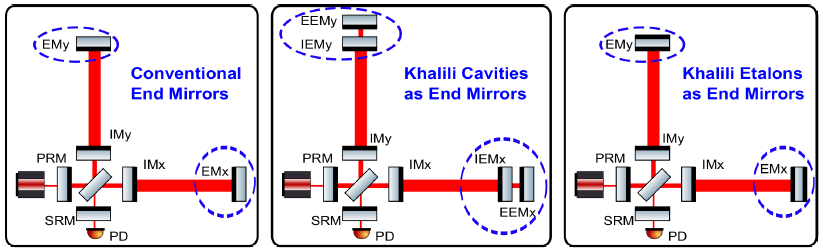
\includegraphics [width =0.85\linewidth]{./Sec_Optics/khalili.png}
\caption {Schematic of an interferometer using a conventional mirror (left), Khalili cavity (middle) and Khalili etalon (right).}\label{fig:khalili_RD}
\end{center}
\end{figure}

In a conventional mirror of an interferometric gravitational wave detector coating Brownian noise is the most dominating noise contribution. The coating Brownian noise is proportional to the mechanical loss as well as the thickness of the coatings layer. In a Khalili cavity the front mirror---where the laser beam senses thermal noise of the cavity---only contains a relatively thin coating. Hence the coating Brownian noise is smaller than a conventional mirror having the same reflectivity.

Keeping the Khalili cavity in its anti-resonant state involves complex control schemes which enhance the complexity of the total interferometer significantly. An alternative approach was proposed \cite{Somiya2011} where instead of using a cavity an etalon will be used (see fig.~\ref{fig:khalili_RD}). This etalon can be thermally length controlled which simplifies the control. Additional noise sources like thermo-refractive noise and mechanical coupling between the two reflective coatings on the different ends of the etalons have been analysed and shown to be small enough to still lead to a thermal noise improvement compared to the conventional mirror.

A detailed analysis of the technical usability of a Khalili etalon is underway and upcoming experiments will demonstrate the usefulness of this approach.

\FloatBarrier
\subsubsection{Coating research}
\label{sec:coating_RND}
%\emph{Author(s): I. Martin, R. Nawrodt}

While silica:Ti-doped tantala coatings have thus-far proven to have the best combination of mechanical loss and optical properties at room temperature, the dissipation peaks in these materials at temperatures below 35\,K are likely to reduce the improvement in coating thermal noise obtained from low temperature operation. Research into possible alternative coating materials is therefore ongoing. Hafnia ($\mathrm{HfO_2}$) may be of particular interest as an alternative high index material as initial measurements have shown a significantly lower mechanical loss than tantala at temperatures below 150\,K~\cite{abernathy11,chalkley10}, although these coatings were found to have high optical absorption due to partial crystallisation. Crystallisation can be prevented by doping hafnia with silica, and there is evidence that this doping does not significantly affect the loss at room temperature. Further studies of the effects of heat-treatment and doping on the mechanical loss and optical properties of hafnia coatings are planned to assess the suitability of this material as a replacement of tantala.

Amorphous silicon can be used as the high-index component of a reflective coating suitable for use at 1550\,nm. Experiments have shown that amorphous silicon coatings deposited by e-beam evaporation can have losses in the order of $10^{-5}$, and that the low-temperature loss can be reduced by more than an order of magnitude by hydrogenation~\cite{liu98}. Additionally, the high refractive index of silicon reduces the number of layers needed for the same reflectivity. In order to achieve the same reflectivity in like a tantala-silica coating of 18 $\mathrm{\lambda/4}$ doublets there are only 6 doublets of silicon-silica needed. Thus, the amount of coating material can be strongly reduced. Thus silicon may be a promising coating material for further investigation, potentially allowing for significant reductions in coating thermal noise. However, additional research is required. There are indications that the silicon-silica interface is chemically not stable. Oxygen starts diffusing from the silica into the silicon forming a silicon mono-oxide boundary layer. This layer might change the optical properties (reflectivity, scattering) of a potential HR stack made from these materials. Thus, a detailed investigation of optical properties of silicon-based optical coatings is required preferably at the desired operational temperature of the ET-LF detector at around 10\,K.

Recent results have strongly indicated that the mechanical loss of coating materials may be strongly related to the local atomic structure. Various techniques are being used to study the structural properties of amorphous coating materials. One technique using electron diffraction Reduced Density Function (RDF) analysis and amorphous modelling allows models of the atomic structure to be obtained from experimental data~\cite{Bassiri2011}. Initial results for tantala coatings indicate increased ordering of the tantala structure as the heat-treatment temperature rises, and it seems likely that these changes may be responsible for the loss peaks observed to occur at higher heat-treatment temperatures. This work is ongoing, with the aim of developing a full understanding of the relationship between the coating atomic structure and the mechanical loss. A better understanding of the mechanical loss processes will influence the final coating choice (exact doping concentration, post-deposition treatment, annealing, etc.).

%\emph{Author(s): J.Franc}\\
In a next future influence of annealing effect on high refractive index material should be tested.
To know more about thin films and substrate materials at cryogenic temperatures, their mechanical losses and absorption investigations must be studied. Previous researches of standard coatings (Ti:Ta$_2$O$_5$ and SiO$_2$) have shown that the mechanical losses of both materials increase at 10\, K compare to the value at 300\,K. %~\cite{Martin200X}. 
Research of other coating materials must be also developed to validate the usual $\mathrm{Ti:Ta_2O_5}$ and $\mathrm{SiO_2}$ thin films. Study of $\mathrm{HfO_2}$, for example, was carried out at Glasgow. Several institutions participate to the mechanical losses measurement for different bulk and coating materials. The sharing of results between the different laboratories will permit to confirm the values and to develop a pretty good database of different materials. Finally, measurement of the silicon $dn/dT$ parameters is also intended. Previous study gave this data at 30\,K at 1500\,nm [already cited], but not below. To know this value will guarantee the exact value of Substrate Thermo Refractive Noise of Silicon, which is, to date, only estimated.

Another point is the estimation of the influence of the coating on reflectivity and thermal noise. A first study performed with the software \emph{TFCalc} for designing and manufacturing optical thin film coatings has demonstrated that a stack of 19 doublets of $\mathrm{Ti:Ta_2O_5}$ and $\mathrm{SiO_2}$ on a silicon substrate corresponds to a transmission of 4\,ppm at a working wavelength of 1550\,nm. The exact coating is $(HL)\_{19}HLL$ with H which corresponds to a high refractive index thin film (2.059 at 1550\,nm) and L for the low refractive index thin film (1.4395 at 1550\,nm).

\begin{figure}
\begin{center}
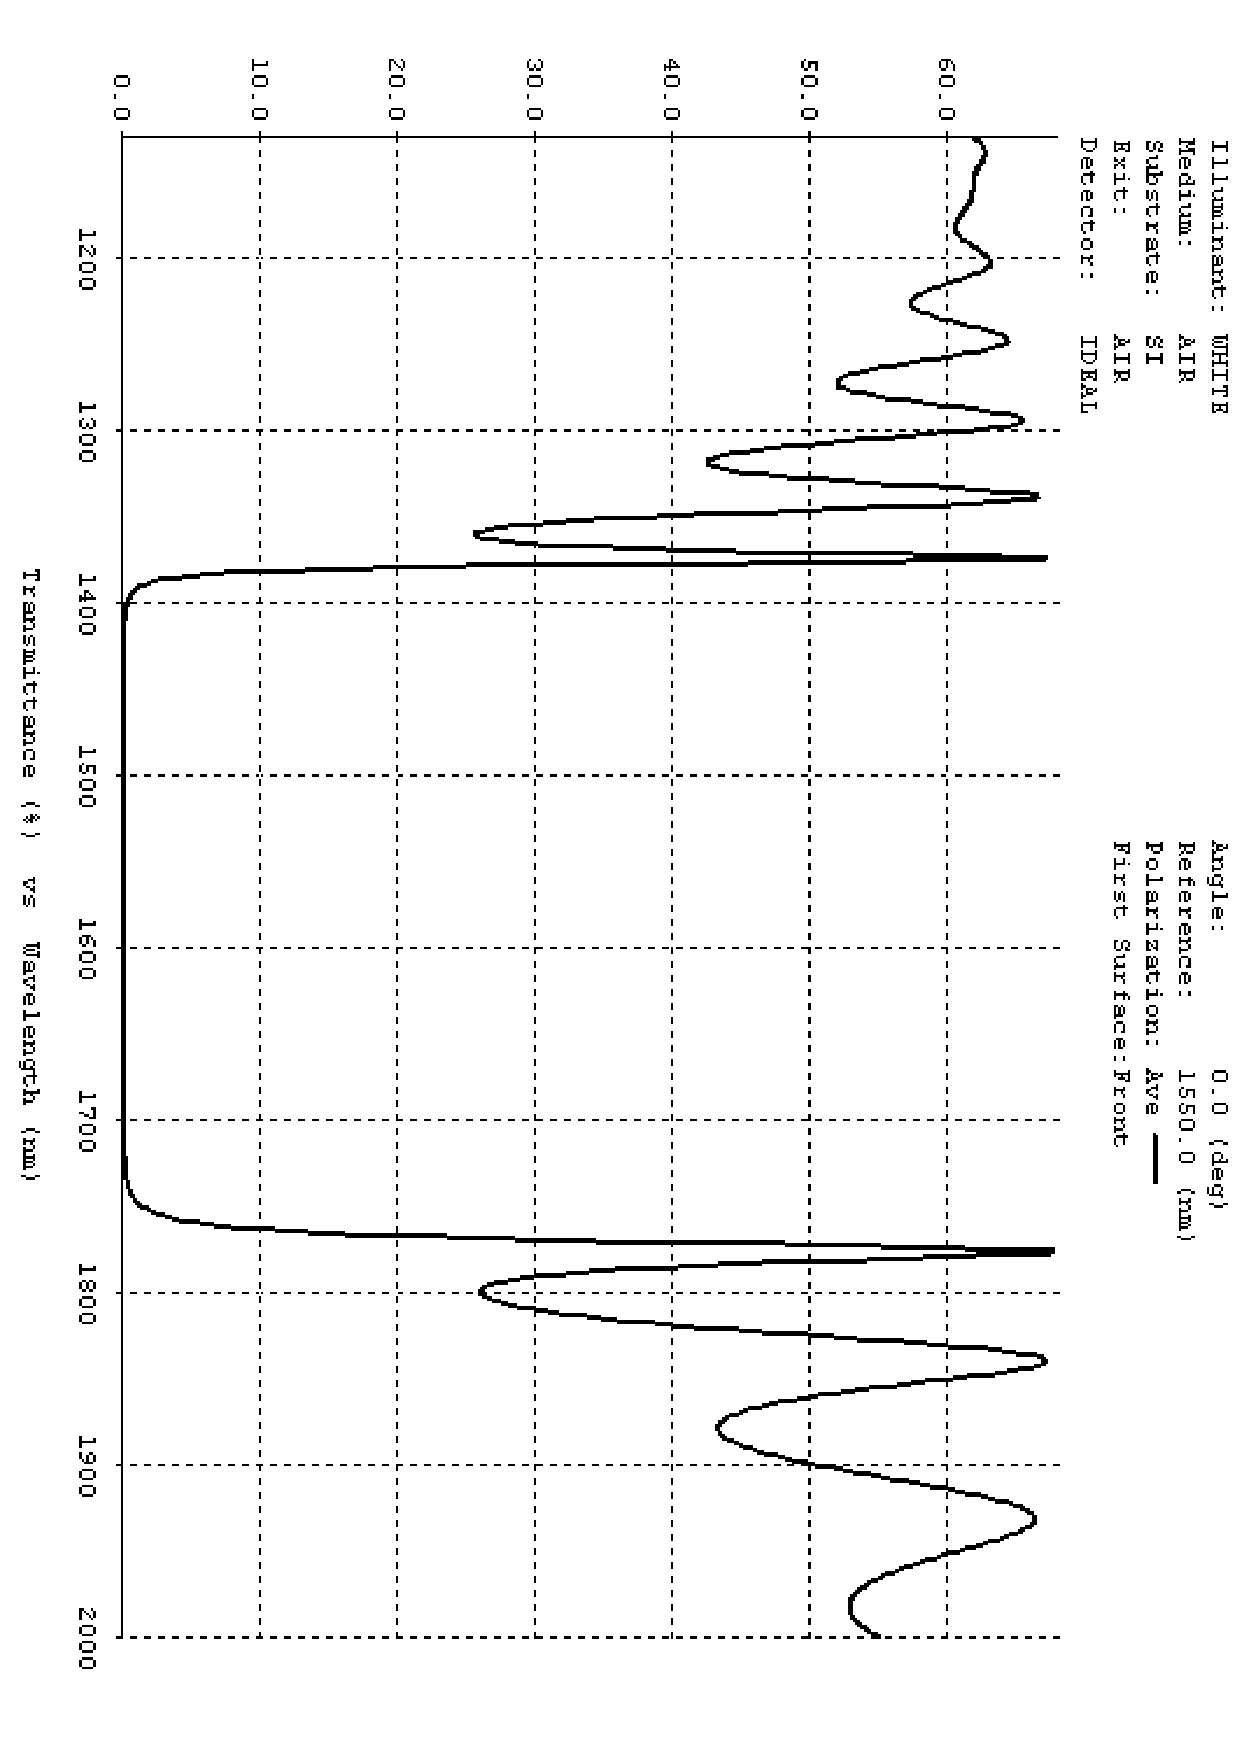
\includegraphics [scale =0.4, angle=90]{./Sec_Optics/HB19HBB.pdf}
\caption {Transmission of stack $HB_{19}HBB$ on a silicon substrate vs wavelengths.}\label{fig:stack}
\end{center}
\end{figure}

Figure~\ref{fig:stack} describes the transmission of a stack $HB_{19}HBB$ on a silicon substrate versus a large range of wavelengths (the figure has been created with the software TFCalc). 

\FloatBarrier
\subsubsection{Waveguide grating mirrors}
%\emph{Author(s): D. Friedrich  }

% Introduction
Test mass mirrors used in gravitational wave detectors are subject to several sources of thermal noise. A dominant contribution is given by Brownian thermal noise caused by mechanical loss of the high reflective multilayer coatings. These, conventionally, are made of up to 20 double layers of tantala (Ta$_2$O$_5$) and silica (SiO$_2$) each having a quarter wavelength optical thickness. Hence, concepts for a reduction of the mechanical lossy materials or for coating free mirrors are being investigated to provide alternative mirror architectures, in order to improve a detector sensitivity in its mid frequency band. For this purpose broadband waveguide grating (WG) structures have been proposed \cite{Bunkowski2006a}, which are based on resonant excitation of light fields in a nanostructured surface that theoretically allow for a perfect reflectivity under normal incidence, without implementing  multilayer stacks.

The basic principle of WGs is shown in Fig.~\ref{fig:WG} using a ray picture~\cite{Rosenblatt97}.

\begin{figure}
\centering
\includegraphics[scale =0.45]{./Sec_Optics/allGWG.pdf}
\caption{Single layer and monolithic waveguide grating architectures.}
\label{fig:WG}
\end{figure}

WGs are basically constructed of a substrate with low index of refraction $n_\mathrm{L}$ and  a nanostructered layer having a higher index of refraction $n_\mathrm{H}$. The grating can be designed such that only specular reflection and three transmitted orders exist. The first order beams in the nanostructured layer are totally reflected at the substrate and partially coupled out at the surface. By adjusting the grating dimensions (optical properties) the outcoupled light fields can be forced to interfere constructively giving a perfect reflectivity.   For dielectric materials Rigorous-Coupled-Wave Analysis (RCWA)~\cite{Moharam1981} is a numerical method to investigate the optical properties of WGs, depending on their material and geometrical parameters, and was used to optimize waveguide gratings in terms of parameter tolerant designs.

It was found that even a zero waveguide layer thickness (only ridges on top of a substrate) can show high reflectivity~\cite{Bunkowski2006a}, which has experimentally been demonstrated using tantala ridges on a silica substrate for the prominent wavelength of $1064\,$nm~\cite{Bruckner2009}. The fabricated waveguide grating (see Fig.~\ref{fig:WG}) was incoporated as a coupling mirror into a linear Fabry-Perot cavity together with a conventional high-reflectivity mirror. From the measured finesse of $\approx 660$ the reflectivity of the waveguide grating was determined to be $(99.08\pm 0.05)\,\%$.

Recent theoretical work~\cite{Bruckner2009} has shown that monolithic waveguide grating structures are also feasible by etching a T-shaped structure into a substrate (see Fig.\ref{fig:WG}). Here, the lower grating is chosen to have a small fill factor (ratio of groove width to grating period) to act as an effective low index medium.
This structure has been fabricated in silicon aiming at a high reflectivity for a laser wavelength of $1550\,$nm. Two etching steps were applied. In the first step the upper grating was defined via anisotropic etching and then protected on its sidewalls. In the second step, an isotropic etching was used to realize the low fill factor grating beneath. The reflectivity was determined in a table-top cavity setup to be $(99.79\pm 0.01)\,\%$~\cite{Bruckner2010} in full agreement with numerical simulations (RCWA)~\cite{Moharam1981}.

While the thermal noise models for conventional multilayer coatings and material parameters are well studied, the thermal noise performance of nanostructured surfaces is still to be investigated. It was experimentally shown that a nanostructured surface does not affect the mechanical quality of a substrate significantly \cite{Nawrodt2007}. However, the mechanical loss and other material parameters such as thermal conductivity of a nanostructure need to be further investigated in order to estimate the actual level of thermal noise. Also a direct measurement of thermal noise of a WG compared to a multilayer coating is of great interest.

Further, the fabrication process needs to be improved to meet the requirements for test masses used in gravitational wave detectors. Besides the optical quality in terms of high reflectivity and homogeneity over the grating area, techniques have to be developed to handle actual substrate dimensions. One approach being investigated is the bonding of a thin nanostructered wafer on a thick substrate.


%Rosenblatt D, Sharon A and Friesem A A,
%IEEE J. of Quantum Electronics 33 (11), 2038–2059(1997)

% Bunkowski06
%Bunkowski, A.; Burmeister, O.; Friedrich, D.; Danzmann, K. & Schnabel, R.
%High reflectivity grating waveguide coatings for 1064 nm
%Classical and Quantum Gravity, 2006, 23, 7297-7303

% Brueckner2009
%Brueckner, F.; Friedrich, D.; Clausnitzer, T.; Burmeister, O.; Britzger, M.; Kley, E.-B.; Danzmann, K.; Tuennermann, A. & Schnabel, R.
%Demonstration of a cavity coupler based on a resonant waveguide grating
%Optics Express, 2008, 17, 163

% Nawrodt07
%R. Nawrodt, A. Zimmer, T. Koettig, T. Clausnitzer, A. Bunkowski, E.-B. Kley, R. Schnabel, K. Danzmann, W.
%Vodel, A. Tueunnermann, and P. Seidel,
%Mechanical Q-factor measurements on a test mass with a structured surface
%New J. Phys. 9, 225 (2007).

% Moharam1981
%RCWA
%Rigorous coupled-wave analysis of planar-grating diffraction
%M. G. Moharam and T. K. Gaylord
%J. Opt. Soc. Am, Vol. 71, Issue 7, pp. 811-818 (1981)

% Brueckner08b
% Opt. Lett. 33,264-66 (2008)
% Monolithic dielectric surfaces as new low-loss light-matter interfaces
% Bruckner et al

% Brueckner10
% Phys. Rev. Lett 104, 63903 (2010)
% Realization of a monolithic high-reflectivity cavity mirror from a single silicon crystal
% Bruckner et al
\FloatBarrier
\subsubsection{Speedmeter topology}

%\emph{Author(s): \textbf{K.\ Kokeyama} and H.\ Mueller-Ebhardt \\}
As mentioned in Section~\ref{sec:qnr},
speed meters can be considered for the ET interferometer
due to their advantage in surpassing the quantum noise limit broadly in the low frequency region.
However, little practical experience of speed meter technology has been accumulated,
in contrast to well-studied Michelson-interferometer (MI) -type position-meter
with currently operated gravitational-wave detectors.
Practical speed meter characterization such as quantum noise surpass-ability
and a capability to optical losses have to be examined in order to select the ET topology.
%Also, the filter cavity technology for variational output which may be inplement on the speed meters
%to enhance the quantum-noise surpass ability
%has not practically investigated well yet,
%(as well as of position-meters).

Speed-meters are realized by either MI-type or Sagnac-interferometer (SI) -type topology,
and only a small part of them is experimentally demonstrated:

\paragraph{Michelson-interferometer type}

\begin{figure}
\centering
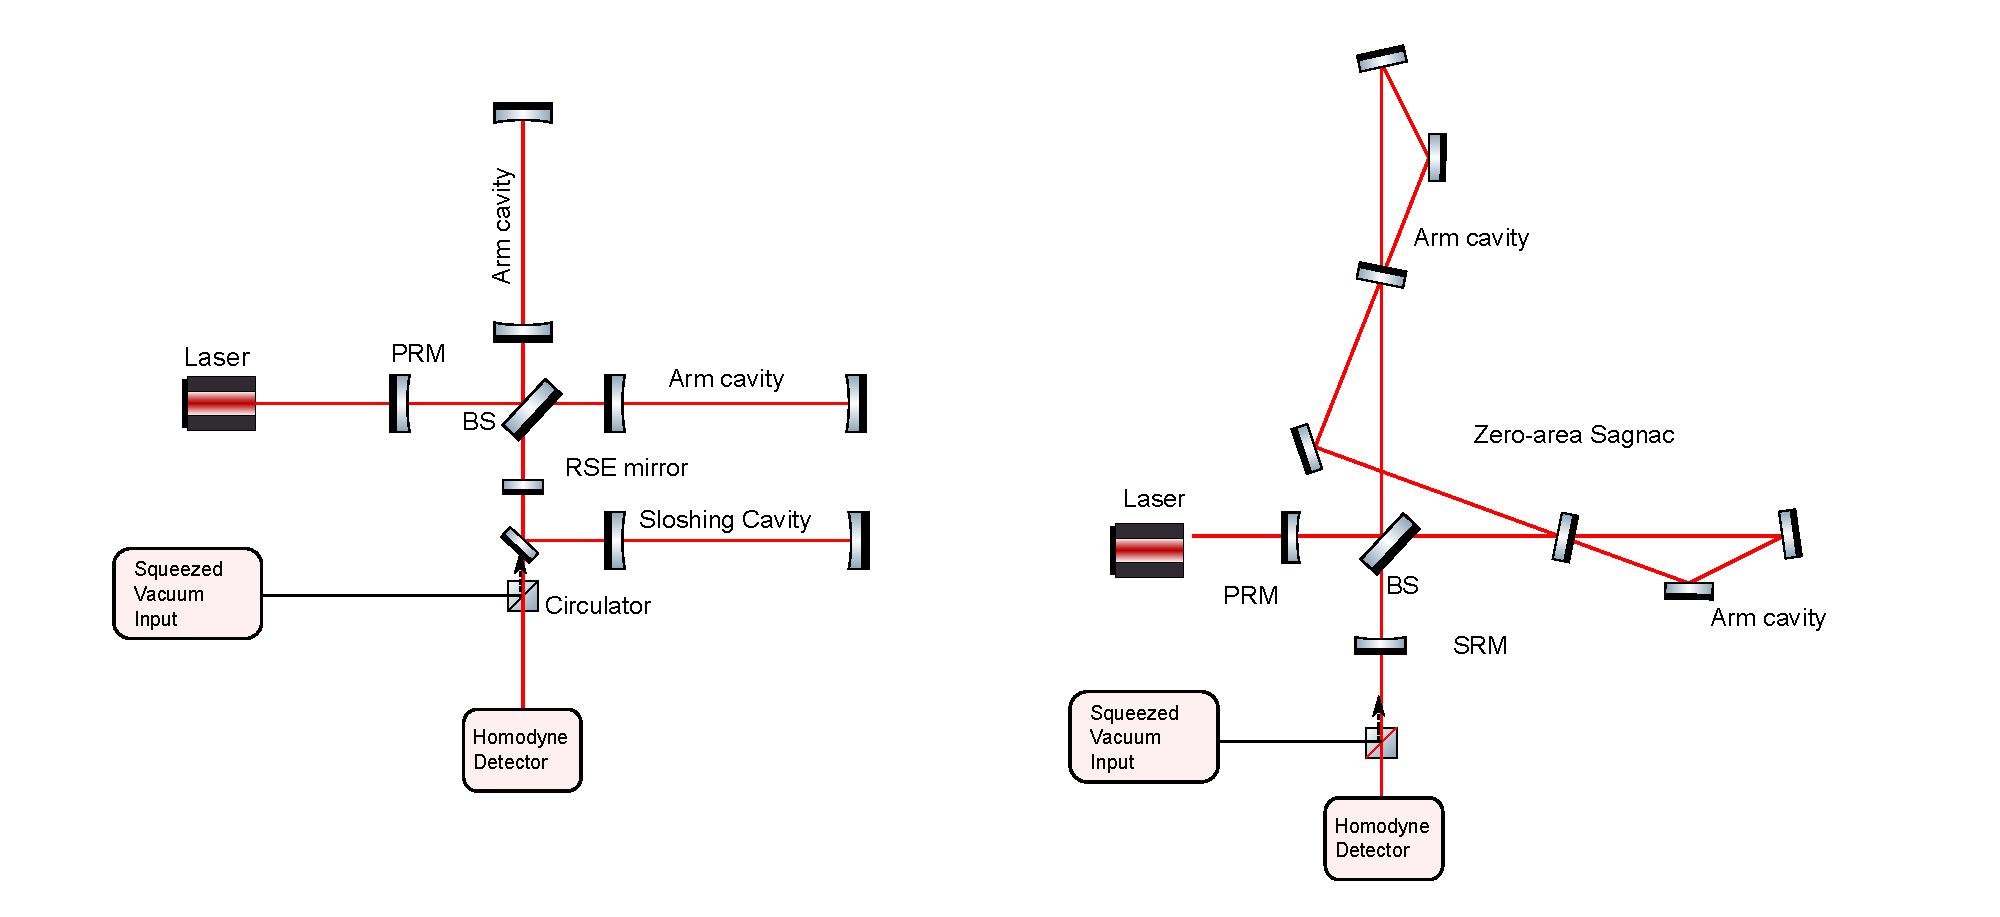
\includegraphics[scale =0.5]{./Sec_Optics/sec5-10-MISM.pdf}
\caption{Left panel: An example configuration of a Michelson-interferometer-type speed meter.
Right panel: An typical configuration of a Sagnac-interferometer-type speed meter
with two ring cavities.}
\label{fig:tech-MISM}
\end{figure}
A typical configuration of a MI type speed meter \cite{Purdue2002, Purdue2002a}
is depicted in the left panel in Fig~\ref{fig:tech-MISM}.
The configuration employs an RSE interferometer with the sloshing cavity at the anti-symmetric port.
The south port of the RSE part is kept to be the dark fringe
(destructive interference between the north and east arms).
When the end mirror of one cavity moves, some light goes through to
the south port, and enters into the sloshing cavity.
The light comes back from the sloshing cavity
and enters the RSE part from the south port. This field is 180 degrees different in phase
and cancels the position information, leaving only the phase shift proportional
to the relative velocity of test masses.
The sloshing cavity adds more complexity such as
the length and alignment degrees of freedom to be controlled,
compered with an RSE topology whose technology is mature and already being installed
in, e.g., Advanced LIGO. Therefore, it is necessary to examine the practical capability of ET.

%% Squeezed vacuum can be applied
%Squeezed-vacuum is injected into the speed meter from the south port
%(squeezed-input speed meter).
%% variational out put option
%Adding two filter cavities to the output port to attain variational output
%is considered as an option (squeezed-variational speed meter).

% what is the MI-SM with polarization optics ?


\paragraph{Sagnac-interferometer type}

The SI-type speed meter~\cite{Chen2003} is depicted in the right panel in Fig.~\ref{fig:tech-MISM}.
A SI is an more straightforward way to realize a speed meter than the MI-type.
A basic SI is a ring interferometer (see the middle panel in Fig.~\ref{Fig:Lshape}
in section~\ref{sec:georeview}) and it is a speed meter by itself.
The laser light is split into two paths by a beam splitter,
then one of the two light fields propagates the ring path in a clockwise direction
whereas the other propogates in a counter-clockwise direction. These two fields interfere at the same beam splitter.
The two fields experience the same path but at different timing depending on the path differences.
Therefore the interference intensity depends only on the time dependent part of the test masses.
For an ET topology, a zero-area SI in which the area enclosed by the two
counter-propagating beams is zero, will be preferable
because it is insensitive to the interferometer rotation.

Before it was realized that the speed meter is free from the quantum back-action noise,
a Sagnac interferometer was investigated
as a candidate topology for the ground based gravitational-wave detectors.
The shot-noise-limited phase sensitivities were demonstrated
by~\cite{Sun1996} and \cite{Beyersdorf02} at high or low frequency region, respectively.

%QND
The squeezed-vacuum will be necessary to be injected from the dark port
to enhance the ability for surpassing the SQL in the broadband frequency region.
This technique has been already demonstrated experimentally
for a zero-area Sagnac interferometer by a table-top experiment~\cite{Eberle2010}.
The non-classical sensitivity improvement of up to 8.2\,dB with
a simple zero-area Sagnac interferometer was experimentally verified.


